\documentclass[11pt]{article}
\usepackage{amsmath}
% use UTF8 encoding
\usepackage[utf8]{inputenc}
% use KoTeX package for Korean
\usepackage{kotex}

\usepackage{hyperref}

\usepackage{graphicx}

\hypersetup{
    colorlinks=true,   
    urlcolor=red,
}

\title{정원 관리를 위한 스마트 플랫폼 개발}

\author{Minwoo Jung}

\begin{document}

\maketitle

\indent \\스마트팜에서 가장 중요한 부분은 적절한 토양 선정과 정확한 관수 주기 조절이다. 토양은 일반적으로 질토, 양토, 사토로 나눌 수 있다.
질토는 진흙으로만 이루어진 토양을 말하며, 흙의 입자가 조밀하고 부드러워 지력이 좋다. 작물 성장 입장에서는 튼실하게 자라지만, 성장이 느리다. 수분 저장력이 높아서 가뭄에 강하다. 유기물의 저장력이 좋아서 초기 생장은 느리지만 점차 성장속도가 빨라진다.
양토는 흙의 입자가 질토와 사토 중간 형태의 적당한 크기이다. 지력이 보통이하로 좋지 않아 작물 생장속도는 평균 이하이다. 수분이나 유기물 저장력 또한 평균적이어서 초기 생육은 좋지만, 점점 생장속도가 저하된다.
사토는 흙의 입자가 굵고 거칠어서 지력과 저장력이 좋지 않다. 초기 생장은 아주 좋지만, 결실을 맺기 어렵다. 
모세관 현상은 지하수가 있는 곳에서 흙의 입자 사이를 비집고 수분이 올라와서 공기 중으로 증발하게 되는 현상이다. 


\begin{figure}[!htbp]
    \centering
       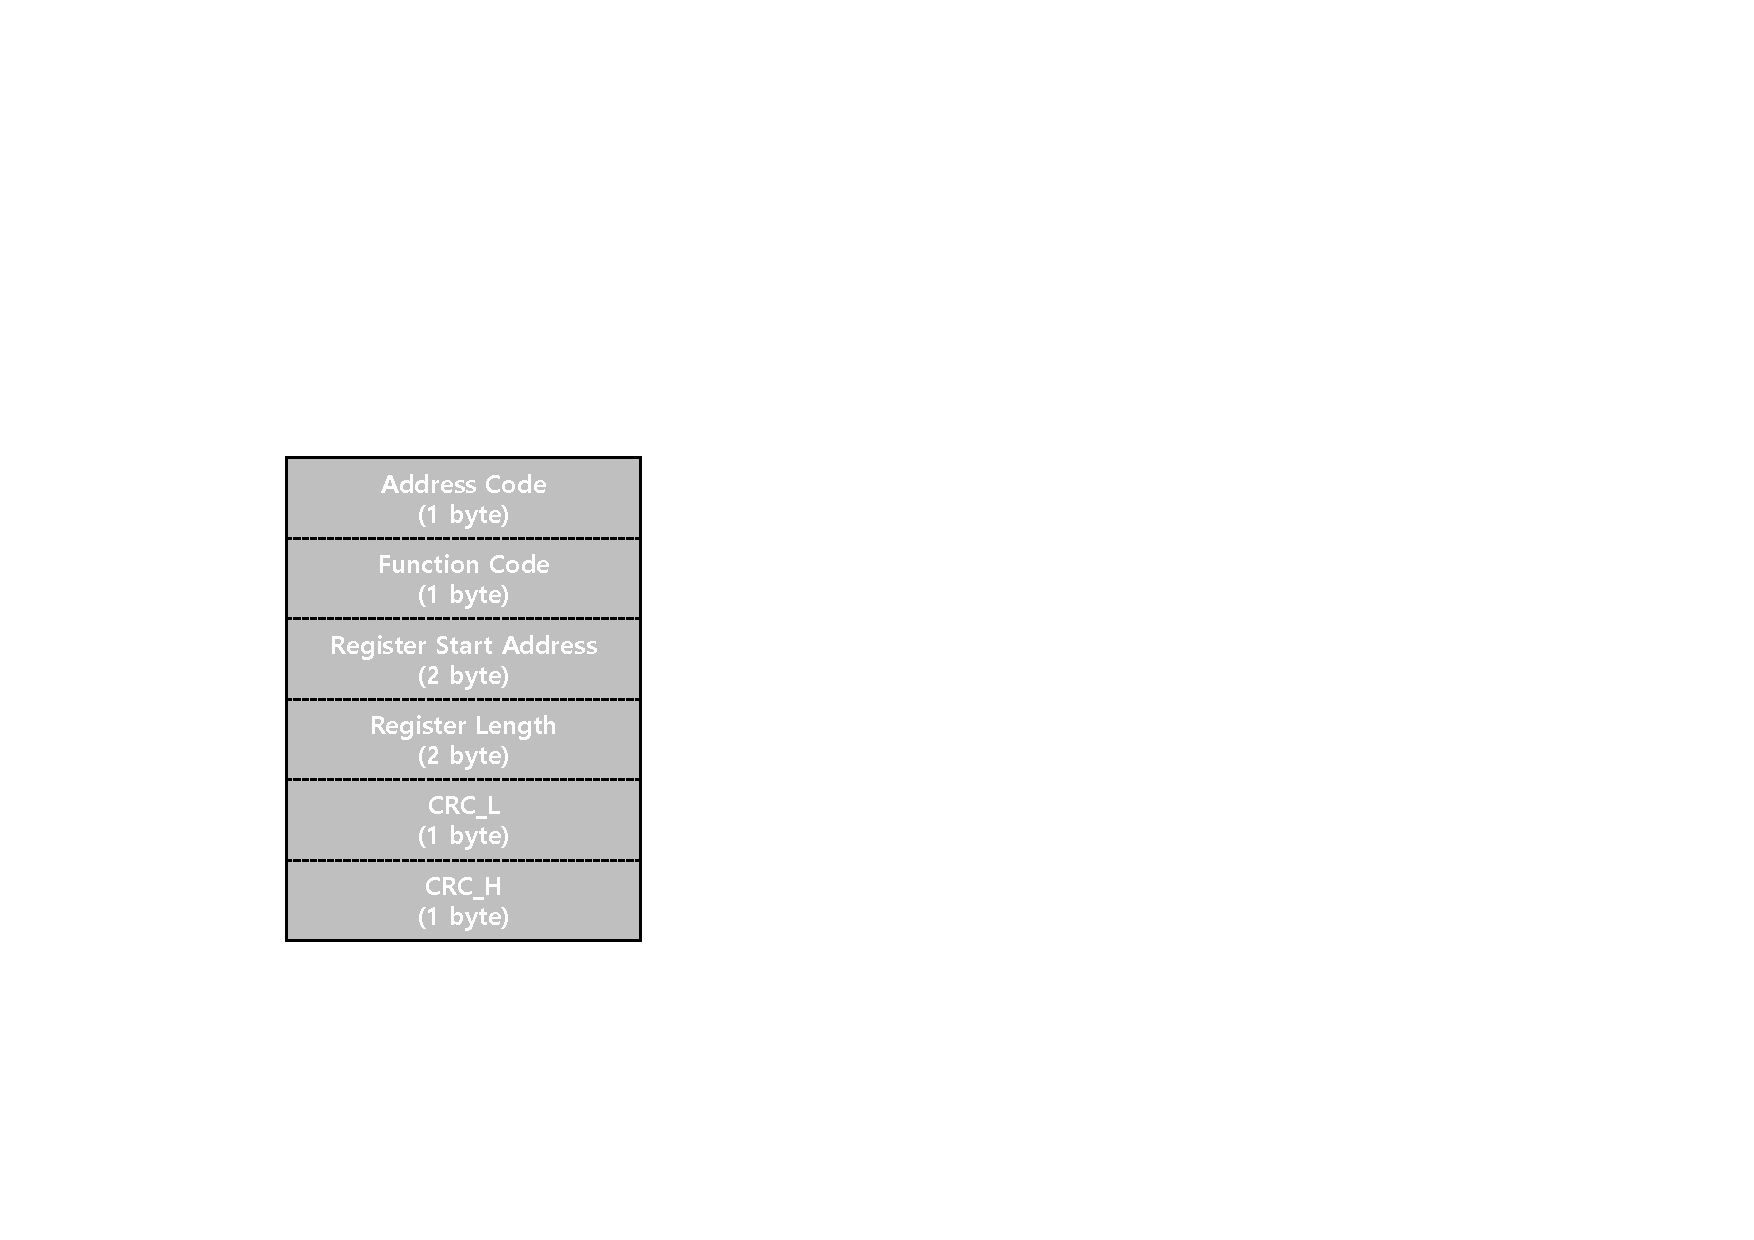
\includegraphics[width=8.5cm]{../Figure/Frame_format.pdf}
       \hfil
    \caption{Data Frame}
    \label{Data_Frame}
\end{figure}

토양센서를 기반으로 토양의 성질을 딥러닝을 기반으로 분석하여 토양 종류를 구분할 수 있다. 토양성분 분석을 통하여 작업 스케줄링을 적응형으로 작성할 수 있다. 

\indent \\

\end{document}
